Addition is the strongest predictor of held-out doubles, and GEARS trained on singles has
more than twice its error. All results use the 131 held-out doubles (GEARS: 128 and 71, explained below) and 5
random half-splits,
with per-pair results averaged over splits. GEARS used seed 1 and 20 epochs in each regime.

\noindent\textbf{Baselines and GEARS joint prediction.} Addition wins on every metric
(\Cref{tab:main} and \Cref{fig:hier}). Denoising the singles makes it worse: low-rank addition beats
plain addition on only 23 of 131 pairs.

\begin{table}[htb]
\centering
\small
\setlength{\tabcolsep}{4pt}
\begin{tabular}{lrccc}
\toprule
Predictor & Pairs & MSE, top-20 DEGs $\downarrow$ & \pd, all genes $\uparrow$ & \pd, top-20 DEGs $\uparrow$ \\
\midrule
\textbf{Additive} & 131 & \textbf{0.081} [0.067, 0.096] & \textbf{0.873} [0.857, 0.886] & \textbf{0.959} [0.952, 0.964] \\
Low-rank additive & 131 & 0.140 [0.123, 0.158] & 0.789 [0.766, 0.810] & 0.870 [0.847, 0.891] \\
GEARS, strict split & 128 & 0.181 [0.161, 0.204] & 0.673 [0.645, 0.700] & 0.862 [0.833, 0.888] \\
GEARS, standard split & 71 & 0.232 [0.194, 0.271] & 0.605 [0.558, 0.653] & 0.798 [0.740, 0.851] \\
Train mean & 131 & 0.575 [0.494, 0.656] & 0.533 [0.488, 0.575] & 0.644 [0.582, 0.700] \\
No change & 131 & 0.734 [0.643, 0.824] & undefined & undefined \\
\bottomrule
\end{tabular}
\caption{Main result on held-out doubles, mean [95\% bootstrap CI over pairs]. The
\addnull beats every other predictor on every metric, and GEARS has more than twice its
error. No-change predicts zero shift, so its correlation is undefined.}
\label{tab:main}
\end{table}

\begin{figure}[htb]
\centering
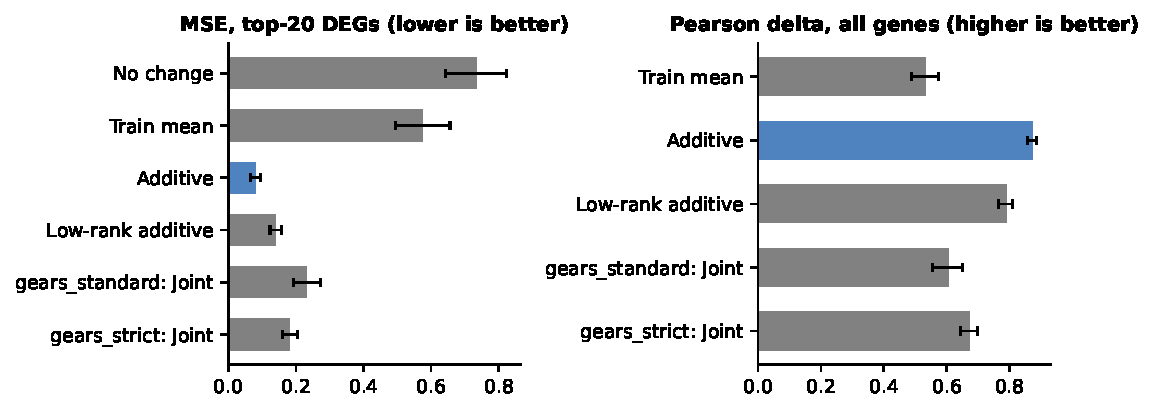
\includegraphics[width=\linewidth]{figs/fig2_null_hierarchy.pdf}
\caption{Baselines and GEARS joint prediction on held-out doubles, with 95\% bootstrap
intervals. Addition (blue) has the lowest error and the highest \pd.}
\label{fig:hier}
\end{figure}

GEARS is scored on fewer pairs for two reasons. Three doubles contain a gene outside GEARS's
gene-ontology graph (IER5L+LYL1, RHOXF2BB+SET, RHOXF2BB+ZBTB25), and on its standard split
GEARS also trains on 57 doubles, which are excluded. On the same pairs, addition scores
0.082 (128 pairs) and 0.085 (71 pairs), so the gap is not a pair-set artefact. On the strict
split, GEARS's MSE exceeds addition's by 0.100 [0.077, 0.122], and GEARS is better on only
14\% of pairs; on the standard split the gap is 0.148 [0.106, 0.187], with GEARS better on
13\%. The two GEARS rows are not directly comparable, because the standard set includes
pairs with a single never seen in training.

\noindent\textbf{Non-additivity is a reproducible property of each pair.} $\eta$ measured on
two disjoint cell halves agrees with Spearman 0.944 (per seed 0.932 to 0.955;
\Cref{fig:eta}). The cross-half estimate of true $\eta^2$ is positive for 99.5\% of pairs
and accounts for 61\% of measured $\eta^2$, so $\eta$ is mostly signal, with a noise share
of about 40\%.

\begin{figure}[htb]
\centering
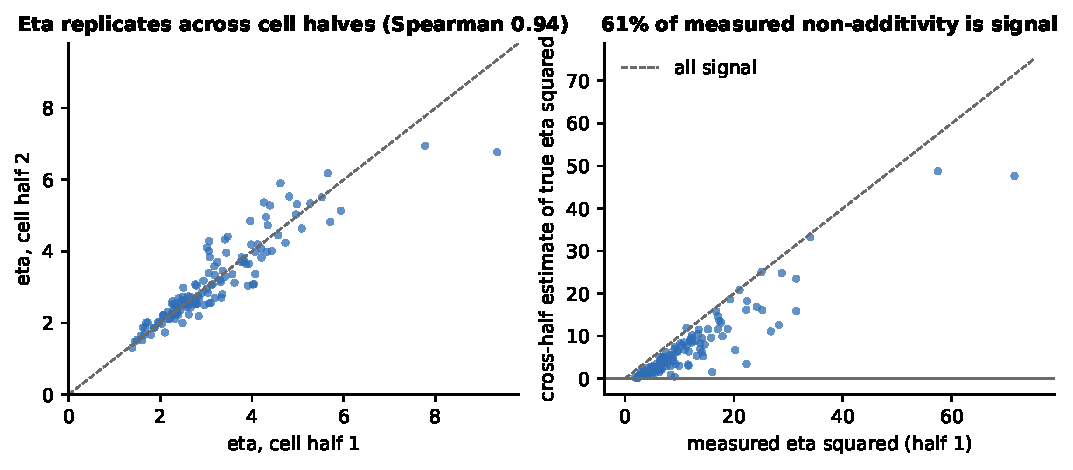
\includegraphics[width=\linewidth]{figs/fig1_eta_reliability.pdf}
\caption{Non-additivity replicates across disjoint cells. Left: $\eta$ on cell half 1 vs.\
half 2. Right: cross-half estimate of true $\eta^2$ vs.\ measured $\eta^2$; the dashed line
is ``all signal''.}
\label{fig:eta}
\end{figure}

\noindent\textbf{Additive error rises with non-additivity.} With $\eta$ from half 1 and error
from half 2, $\eta$ and additive MSE correlate with Spearman 0.82 across pairs
(\Cref{fig:addeta}). Additive error rises about fivefold from the low to the high tertile;
GEARS stays above it throughout, and the gap narrows only where interactions are strongest
(\Cref{tab:tert}). The most non-additive pairs are dominated by the CEBP family
(CEBPA+CEBPB, CEBPA+CEBPE, CEBPE+SET, CEBPA+KLF1), consistent with the redundant
differentiation programmes Norman et al.\ described.

\begin{figure}[htb]
\centering
\begin{minipage}{0.52\linewidth}
\centering
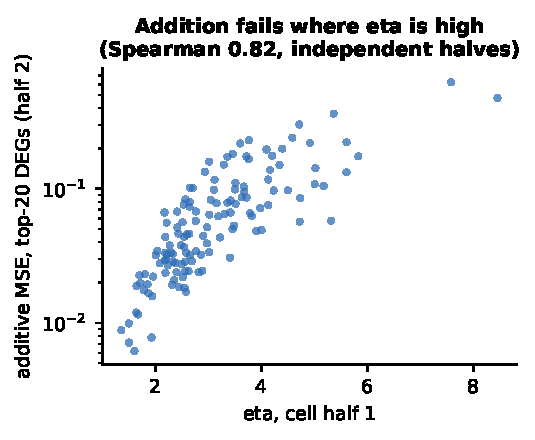
\includegraphics[width=\linewidth]{figs/fig3_additive_vs_eta.pdf}
\captionof{figure}{Additive error (half 2) against $\eta$ (half 1), one point per double.}
\label{fig:addeta}
\end{minipage}\hfill
\begin{minipage}{0.44\linewidth}
\centering
\small
\begin{tabular}{lcc}
\toprule
$\eta$ tertile & Additive & GEARS strict \\
\midrule
Low & 0.028 & 0.140 \\
Mid & 0.064 & 0.210 \\
High & 0.153 & 0.194 \\
\bottomrule
\end{tabular}
\captionof{table}{MSE on the top-20 DEGs by $\eta$ tertile, same 128 doubles. GEARS is worse
than addition in every tertile.}
\label{tab:tert}
\end{minipage}
\end{figure}

\noindent\textbf{Round-trip gate.} Strict GEARS passes on the 5 singles with the most cells
(KLF1, BAK1, CEBPE, ETS2, UBASH3B). Real $A$-perturbed cells passed through with no new
perturbation come back with $r = 0.999$ on expression and 0.80 to 0.99 on shifts from
control, and its own predicted states behave the same. The pass is structural, not learned:
a second application of $A$ moves the cell exactly as far as the first, so the shift simply
doubles (saturation ratio 1.0 for all five genes). The GEARS source explains why: input expression enters only as a final
residual, $\mathrm{out} = x + g(\mathrm{pert})$, and $g$ ignores the input cell.
